\chapter{تنسيق الصور والجداول بلغة اللتيك}

\section{اهداف الباب}

\section{تنسيق الصور}
معظم الوثائق اليوم تحتوي على الكثير من الصور والجدوال. وهذا النوع من المحتوى يتحتاج الى تنسيق خاص وذلك لان هذه الكائنات ليمكن تجزئتها بين الصفحات عندما نصل الي نهاية الصفحة. فالمعتاد عمله في هذه الحالة هو انتقال الجدول او الصور الى الصفحة التالية وترك جزء من الصفحة السابقة فارغ. في هذه الحالة سوف يظهر تنسيق الوثيقة غير لائق لانه يحتوي على الكثير من الفراغات. لذلك تعمد لغة الليتك الى استخدام حاويات خاصة 
تسمى العوائم floats لتنسيق الصور في الوثائق. وسبب تسميتها بهذا الاسم هو لان هذه العوائم تاجل وضع الجداول والصور لكي تسمح للنص بملأ الفراغات في الصفحات التي لايمكنها احتواء الصور والجدوال. وبعد ذلك يقوم ليتك بوضع العوائم في الوثيقة بعد  ان قام بملأ ما يمكن ملئة من فراعات. وقد يسبب عدم فهم المستخدم لهذه العوائم الكثير من المتاعب لذلك فان استيعابها يعتبر غاية في الاهمية. وكما هو متعارف عليه فأن لكل عائمة تعليق مرقم لوصف العائمة بحيث يساعد الترقيم على الاشارة الى العائمة من اي مكان في الوثيقة. وعدد العوائم محدود ولا يمكن ان يزيد عن ١٨ عائمة في كل وثيقة. ولاضافة صورة في الوثيقة يمكن كتابة الكود التالي:
\begin{english}
\begin{mybox}
\textbackslash begin\{figure\}[\textarabic{محدد مكان الصورة ان وجد}]\\
... \textarabic{محتويات الصورة}...\\
\textbackslash end\{figure\}\\
\end{mybox}
\end{english}
محدد مكان الصورة يعطي المستخدم القدرة على التحكم في مكان الصورة الموضوعة في العائمة ومن خيارات محدد مكان الصورة مايلي:\\
\\
\begin{tabular}{|l | p{11cm}|}
\hline
h & تضع العائمة على مقربة من مكان الكود في الوثيقة\\ \hline
t & تضع العائمة في اعلى الصفحة\\ \hline
b & تضع العائمة في اسفل الصفحة\\ \hline
P & يضع العائمة في صفبحة معينة  \\ \hline
! & text \\ \hline
H & تضع العائمة بالضبط في المكان الذي يختارة المستخدم وهذا الخيار يحتاج الى اضافة مكتبة العوائم
float  \\ \hline
\end{tabular}
\\
\\
لاضافة جدول بقائمة الصور الموجودة في الوثيقة يمكن استخدام الامر التالي في بداية الوثيقة:\\
\begin{english}
\begin{mybox}
\textbackslash listoffigrures
\end{mybox}
\end{english}
لاضافة اطار حول الصورة يجب كتابة الكود التالي في جزء اعدادات الوثيقة:\\
\begin{english}
\begin{mybox}
\textbackslash usepackage\{float\}\\
\textbackslash floatstyle\{boxed\} \\
\textbackslash restylefloat\{figure\}
\end{mybox}
\end{english}
لاضافة صورة للوثيقة يجب استدعاء مكتبة الصور graphicx في جزء اعدادات الوثيقة اولا ثم اضافة الكود التالي للوثيقة:\\
\begin{english}
\begin{mybox}
\textbackslash begin\{figure\}[h]\\
\textbackslash includegraphics\{box\}\\
\textbackslash caption\{This is a box\}\\
\textbackslash label\{box1\}\\
\textbackslash end\{figure\}
\end{mybox}
\end{english}
في الكود السابق تم استخدام الامر 
\textbackslash includegraphics\{\} وذلك لاضافة الصورة الى الوثيقة. ام اسم ملف الصورة فيتم وضعه بين القوسين المتعرجين. فاسم ملف الصورة في المثال السابق هو 
box 
ويجب ملاحظة ان يكون ملف الصورة في نفس مكان ملف الوثيقة والا فان المستخدم يجب عليه ان يحد مكان ملف الصورة بكتابة اسم المجلدات التي تحتوي على اسم الصورة. ويستخدم الامر 
\textbackslash caption\{\} 
كتابة تعليق على الصورة حيث يمكنك كتابة ماتشاء داخل القوسين المتعرجين التي تلي امر التعليق. ويستخدم الامر 
\textbackslash label \{\}
لاضافة مرجع مرقم للصور بحيث يمكن الاشارة الي الصور داخل النص و ذلك باستخدام الامر 
\textbackslash ref\{\}
والمثال التالي وضح كيفية الاشارة الى الصورة من خلال النص:\\
\begin{mybox}
	\begin{figure}[H]
		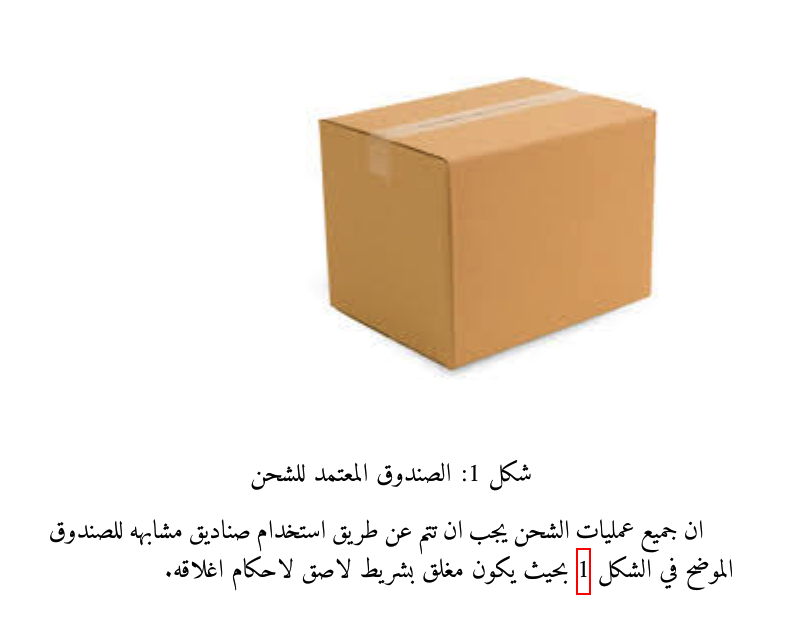
\includegraphics[width=\linewidth]{figures/example2.png}
		\caption{\textarabic{مثال على طريقة استخدام التعليق وطريقة الاشارة اليه في النص}}
		\label{fig:startpython}
	\end{figure}
\end{mybox}